\documentclass[twocolumn,10.5pt,a4]{article}
\usepackage[top=25truemm,bottom=30truemm,left=20truemm,right=20truemm]{geometry}
\usepackage{graphicx}
\begin{document}

\title{Propagation length of mid-infrared surface plasmon polaritons at gold/air interface}
\author{Nobuyoshi Hiramatsu, Fumiya Kusa, Akinobu Takegami, Kotaro Imasaka,  \\Ikki Morichika, Satoshi Ashihara\\ Institute of Industrial Science, the University of Tokyo, \\4-6-1 Komaba, Meguro-ku, Tokyo 153-8505, Japan}
\maketitle

\section{Introduction}
Mid-infrared plasmonics based on metal materials is beneficial for a number of applications including surface-enhanced spectroscopies\cite{Osawa}\cite{Neubrech}, plasmonic circuit\cite{Ebbesen}, chemical sensors\cite{Matthew}, thermal radiation control\cite{Takahara}, and strong field effect\cite{Kusa2015}. 
Their efficiencies and functionalities rely on the degree of electric-field enhancement induced by surface plasmons (SPs), namely, localized surface plasmons (LSPs) and surface plasmon polaritons (SPPs).

The electric-field enhancement is limited by damping or decay rate of the SPs, which comes from either radiative or irradiative damping of the SPs. 
The radiative damping is regarded as coupling with propagating light, that highly depends on the detail of metal shape and size, or the applications. On the other hand, the irradiative damping originates from electron-electron scattering or electron-lattice scattering, which is inherently inevitable for the plasmonic applications. Here, metal morphology is known to be influential for the irradiative loss, which is expressed by its dielectric constant\cite{Jens}\cite{Hunghua}.

Gold is often used for a plasmonic material in visible and mid-infrared range due to its high optical conductivity and stability under ambient condition. Propagation length of SPPs essentially characterized the irradiative damping. 
However, the propagation length of mid-infrared SPPs on gold has not been measured to our knowledge, whereas Shiba {\it et al.} reported on copper\cite{Shiba}.

In this study, we quantitatively investigated the propagation length of mid-infrared SPPs bound to a Au/air interface, by using several sets of a waveguide with different lengths at a wavelength of $10.6\:\mathrm{\mu m}$. 
During the experiment, morphology of the gold waveguide was manipulated by thermal annealing, and measured by atomic force microscopy (AFM). 

The remainder of this paper is organized as follows.
In Sec.~\ref{sec:device}, design and fabrication of the SPP devices are illustrated.
In Sec.~\ref{sec:experiment}, the optical setup and annealing procedure are described.
In Sec.~\ref{sec:result}, the measured propagation length of SPPs and the characterized surface morphology are shown.
In Sec.~\ref{sec:discussion}, we discuss physics underlying our experimental results and we draw conclusions in Sec.~\ref{sec:conclusion}.

\if0
\cite{Kusa2014}
\cite{Olmon}
\fi

\section{Device design and fabrication}
\label{sec:device}
In order to measure the propagation length of SPPs, we designed a series of SPP waveguide devices. Each device consists of an input coupler, an SPP waveguide, and an output coupler.  The input/output coupler is an surface relief grating made of gold. SPPs are  excited at the input coupler from freely-propagating light, propagate along the SPP waveguide, and are re-converted to freely-propagating light at the output coupler, as illustrated in Fig. \ref{fig:Device}(a). 

The ratio of the output power to the input power is determined by light-SPP coupling efficiency, SPP propagation loss, and SPP-light coupling efficiency. If the input/output coupling efficiencies are identical among all devices,  the input-output power ratio directly reflects the propagation loss. In a word, by measuring the input-output power ratio for devices with different waveguide lengths, we can decuce the distance that the SPP power falls to $1/e$ of its initial value, namely, the propagation length. In the experiments described below, we assumed that the coupling efficiencies are idential among all devices and measured the output optical power for each device, while incident optical power kept constant. 

Freely-propagating light and SPPs can be coupled to each other by using a grating structure which satisfies the condition \cite{Koev},
\begin{equation}
k_{\mathrm{SPPgr}}=k_0 \sin \theta + \frac{2m\pi}{d},
\label{eq:phase-match}
\end{equation}
where $k_{\mathrm{SPPgr}}$ and $k_0=2\pi/\lambda_0$ are the wave vector of SPP at the grating and that of light in free space, respectively, $\lambda_0$ is the wavelength of light in free space, $\theta$ is an incident angle, $d$ is a grating pitch, and $m$ is an integer. Here we note that $k_{\mathrm{SPPgr}}$is close to the SPP wavevector on a flat film in the case of shallow gratings.

Grating depth is known to be influential for the light-SPP (SPP-light) coupling efficiency\cite{Koev}\cite{Justin}. 
To find the optimum grating height for the strongest coupling, we conducted numerical simulations on reflection efficiencies of surface relief gratings made of gold, by the rigorous coupled-wave analysis (RCWA)\cite{Leveque}. 

Here, we assumed that each grating is made of polycrystalline gold (please refer to E. D. Palik, Handbook of Optical Constants of Solids (Academic Press, Orlando, 1985)) with a rectangular profile, a grating pitch of $15\:\mathrm{\mu m}$, and a duty cycle of 0.5. We also assumed that incident light is a plane monochromatic wave with a wavelength of $10.6\:\mathrm{\mu m}$. 
Figure \ref{fig:Device}(b) shows the calculated reflection efficiency as a function of incident angle and grating depth. The reflection efficiency reveals a dip at the grating depth $0.2-1.3\:\mathrm{\mu m}$ for the incident angle of 17-18 degree. 
The loss of power in the reflected beam originates from energy conversion from freely-propagating light to SPPs.
Here we set the grating period and the incident angle so as to minimize power loss into diffracted light in free space; there is no diffraction other the specular reflection.  From these numerical results and the possible beam divergence (?degree) of the incident light in our experiments, we predict that efficient coupling would be obtained for the grating depth of $\sim0.8\:\mathrm{\mu m}$. This prediction is consistent with a previous report which concluded that the optimum grating depth of a rectangular grating is 10\%-15\% of the wavelength in mid-infrared range\cite{Justin}.

Figure \ref{fig:Device}(c) shows the design of the waveguide devices, used in our experiments.  The waveguides have a common width of $0.5\:\mathrm{mm}$ and varied lengths of $3, 5, 7, 9,$ and $11\:\mathrm{mm}$. The input (output) coupler is 1 mm in length and $0.5\:\mathrm{mm}$ ($1.5\:\mathrm{mm}$) in width. Both of the input/output couplers have rectangular profiles with a grating pitch of $15\:\mathrm{\mu m}$ and a duty cycle of 0.5. As will be described below, the waveguides and the gratings are fabricated with a common hight of $0.8\:\mathrm{\mu m}$ on a 200-nm-thick gold base layer.

The device was fabricated by means of electron beam lithography, thermal evaporation, and lift-off process. Gold base layer with a thickness of $200\:\mathrm{nm}$ was thermally evaporated on a silica glass substrate with a 5-nm-thick chromium adhesion layer, after the substrate was cleaned with acetone and ethanol. Then, electron-beam resist (OEBR-CAP112PM, Tokyo Ohka Kogyo Co., Ltd) was spin-coated with a thickness of $1700\:\mathrm{nm}$ on the gold base layer, exposed by electron beam, and developed. Finally, gold with a thickness of $800\:\mathrm{nm}$ was deposited on the developed resist, and the resist was lifted off by acetone. The whole fabrication process was conducted at room temperature. During the evaporation, we maintained the evaporation rate of gold to be $0.4\:\mathrm{nm/s}$, and the pressure inside the vacuum chamber to be less than $3\times10^{-5}\:\mathrm{Torr}$. 

 \begin{figure}[!htbp]
   \begin{center}
    \includegraphics[width=\hsize]{./device.eps}
    \caption{(a) Schematic of the SPP device. (b) Calculated reflection efficiency of a gold relief grating with a grating pitch of $15\:\mathrm{\mu m}$ and a duty cycle of 0.5, as a function of the incident angle and the grating depth. (c) Design of SPP waveguide and input/output couplers. THE ORDER HAS BEEN CHANGED!}
     \label{fig:Device}
   \end{center}
\end{figure}

\section{Experiment}
\label{sec:experiment}
Figure \ref{fig:Experiment} shows the schematic of our experimental setup. 
A $\mathrm{CO_2}$ laser was used as a mid-IR light source generating linearly polarized light at a wavelength of $10.6 \:\mathrm{\mu m}$. 
The SP device was attached to a rotational and xyz-translational stage. 
P-polarized light was incident onto the input coupler at a certain angle that fulfills Eq. \ref{eq:phase-match} where $m=1$, being loosely collimated by a spherical mirror with a radius of curvature $R=400\:\mathrm{mm}$. 
Here the incident light converges with an angle as small as ? degree. This plane-like wavefront of the incident light and the homogeneous grating coupler results in a collimated SPP beam which should propagate with low divergence. The SPP beam divergence is extimated to be ? degree and therefore we believe that the excited SPP beam propages freely along the waveguide without horizontal confinement owing to the SPPwaveguide.
The output light was collected by a spherical mirror of $R=150\:\mathrm{mm}$ and a power meter. 
An aperture was placed at the conjugate point of the output coupler. 
The time averaged power of the $\mathrm{CO_2}$ laser was controlled by changing the duty ratio of the RF power modulation.
The optical power sent to the input coupler was typically $60\:\mathrm{mW}$, and the duty ratio was typically $0.5$.
We also used a He-Ne laser as a guide laser, which was collinearly overlapped with the mid-IR light. 

In order to modify the morphology of the gold film, the sample was annealed twice with a hotplate in Argon atmosphere\cite{Nogues}.
In the first annealing process, the sample was heated at $600\:^\circ\mathrm{C}$ for $20\:\mathrm{min}$., and gradually cooled on the hotplate to room temperature. In the second annealing process, the sample was heated at $700\:^\circ\mathrm{C}$ for $16\:\mathrm{min}$., and cooled down in the same way.

Surface morphology was measured by AFM in non-contact mode (DESCRIBE THE PRODUCT NAME AND THE PRODUCTION COMPANY OF THE AFM), and crystal grains were identified by analyzing the height data of the surface based on the watershed algorithm\cite{Petr}.


 \begin{figure}[!htbp]
   \begin{center}
    \includegraphics[width=0.8\hsize]{./Experiment.eps}
    \caption{Schematic of experimental setup.}
     \label{fig:experiment}
   \end{center}
\end{figure}


\section{Results}
\label{sec:result}
Figure \ref{fig:propagation_length} shows the measured output power as a function of the SPP waveguide length $L$ for (a) the as-grown, (b) once-annealed ($600\:^\circ\mathrm{C}$), and (c) twice-annealed ($600\:^\circ\mathrm{C}$ and $700\:^\circ\mathrm{C}$) sample.
Here, each trace ($a\!\sim\!c$) of the output power is normalized by the value at $L=0$, obtained by the least squares fitting with the exponential decay function $\exp(-L/L_{\mathrm{SPP}})$. 
The propagation length $L_{\mathrm{SPP}}$ is evaluated as $9.0\pm0.3\:\mathrm{mm}$, $12.0\pm0.4\:\mathrm{mm}$, and $14.7\pm0.7\:\mathrm{mm}$ for the sample (a), (b), and (c), respectively.
In this way, the propagation length increased by the annealing process.

The SPP-light coupling efficiency of the grating is estimated to be 18\% in the experiment, by calculating a square root of the normalized output power at $L=0$ divided by the input power.
After annealing, optimum incident angle for the maximum excitation efficiency of SPP was shifted by about $0.5^\circ$, but no significant change was confirmed in the value of the efficiency.

Figure \ref{fig:morphology} shows AFM topography images of the surface of SPP waveguides for the sample (a), (b), and (c).
Isotropic deposition of gold and flat surface were confirmed for all samples. 

Surface roughness is estimated to be $5.67\:\mathrm{nm}$, $2.82\:\mathrm{nm}$, and $2.15\:\mathrm{nm}$ for the sample (a), (b), and (c), by calculating two-dimensional root mean squares of deviations in height data. 
The surface roughness decreased by the annealing process.

For detailed characterization of the surface morphology, crystal grains were identified based on the watershed algorithm. Aspect ratio of the grain is calculated as $1.6\pm0.8$, $2.4\pm2.5$, and $2.0\pm1.8$ for the sample (a), (b), and (c), respectively. In the assumption that the grains are close to spherical shape, grain diameter is estimated to be $70\:\mathrm{nm}$, $190\:\mathrm{nm}$, and $180\:\mathrm{nm}$, for the sample (a), (b), and (c), respectively.
In this way, the crystal grain size significantly increased by the first annealing at $600\:^\circ\mathrm{C}$, and remained similar by the second annealing at $700\:^\circ\mathrm{C}$.

The grating structures were not significantly deformed after the annealing. However, pinholes with diameters of $0.3-1.2\:\mathrm{\mu m}$ appeared with a number density of $0.16\:\mathrm{\mu m^{-2}}$ after the first annealing process, and increased to $0.44\:\mathrm{\mu m^{-2}}$ in number density after the second annealing.

 \begin{figure}[!htbp]
   \begin{center}
    \includegraphics[width=\hsize]{./propagation_length.eps}
    \caption{Measured output power as a function of the SPP waveguide length $L$ for (a) the as-grown, (b) the once-annealed ($600\:^\circ\mathrm{C}$), and (c) the twice-annealed sample ($600\:^\circ\mathrm{C}$ and $700\:^\circ\mathrm{C}$). The propagation length of SPP is evaluated as $9.0\pm0.3\:\mathrm{mm}$, $12.0\pm0.4\:\mathrm{mm}$, and $14.7\pm0.7\:\mathrm{mm}$, respectively for the sample (a), (b), and (c).}
       \label{fig:propagation_length}
   \end{center}
\end{figure}

 \begin{figure}[!htbp]
   \begin{center}
    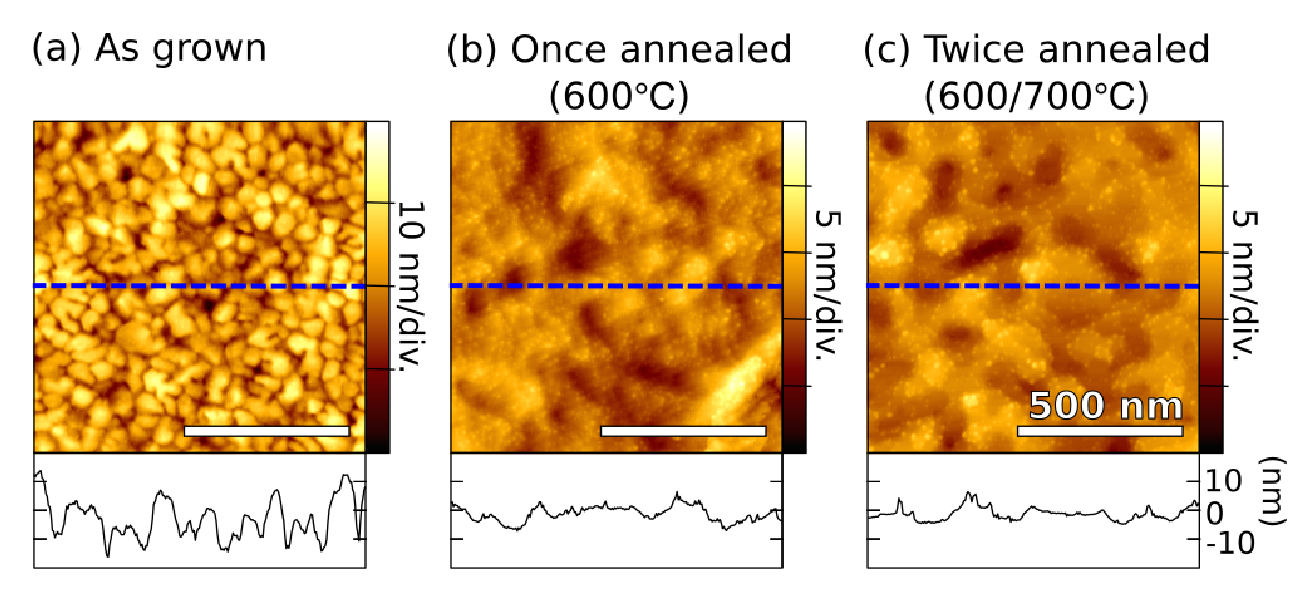
\includegraphics[width=\hsize]{./morphology.eps}
    \caption{Height plots on the surface of waveguides based on AFM.}
    \label{fig:morphology}
   \end{center}
\end{figure}

\section{Discussion}
\label{sec:discussion}
Propagation length of SPP $L_{\mathrm{SPP}}$ at Au/air boundary can be calculated by the following equation,
\begin{equation}
 L_{\mathrm{SPP}} = \frac{1}{2\:\mathrm{Im} k_{\mathrm{SPP}}},
\label{eq:propagation_length}
 \end{equation}
where the wave vector is $k_{SPP}=\lambda/(2\pi\sqrt{\epsilon_g/(\epsilon_g+1)})$, and $\epsilon_g=\epsilon'_g+i\epsilon''_g$ is relative dielectric constants of gold. 
By substituting the dielectric constant of polycrystalline gold\cite{Palik} into Eqn. \ref{eq:propagation_length}, the propagation length of SPP is calculated to be $12.3\:\mathrm{mm}$ at a wavelength of $10.6\:\mathrm{\mu m}$.
Our experimentally measured values of  $9.0\pm0.3\:\mathrm{mm}$, $12.0\pm0.4\:\mathrm{mm}$, and $14.7\pm0.7\:\mathrm{mm}$ agree with the theoretical estimation of $12.3\:\mathrm{mm}$, confirming that SPPs at Au/air interface do propagate for along distance of $>10\:\mathrm{mm}$.

Grain boundaries reduce the mean free path of electrons\cite{Jens}. Therefore, the SPPs loss its energy by introduction of the grain boundaries due to the oscillating electrons, decreasing the propagation length. 
An additional loss mechanism was suggested in \cite{Kuttge}, that SPPs scatter due to inhomogeneities of free electron gas due to grain boundaries. 

Comparing the first annealing at $600\:^\circ\mathrm{C}$ , we find enlargement of the crystal grains, suppression of the surface roughness, and the increased propagation length. Since influence of the grain boundaries become stronger as the averaged grain diameter decreases, we confirmed the longer propagation length of the mid-infrared SPPs in mid-infrared range which is contributed from enlargement of crystal grains.

After the second annealing at $700\:^\circ\mathrm{C}$, although the propagation length increased considerably, the averaged grain diameter does not enlarged, comparing the once-annealed sample and the twice annealed sample. 
This mismatch occurred can be attributed to the reduced aspect ratio of the crystal grains and the deviation. As the aspect ratio decrease, the area of grain boundaries get smaller even if the estimated grain diameter was unchanged. It follows that, averaged number of grain boundaries that the SPPs passing through per a unit length increases, and the mean free path of electron decreases. The reduced deviation results similarly to the area of grain boundaris, thus influences the mean free path of electrons.
In any case, the elongated propagation length was demonstrated by the annealing, which is relevant with the material morphology.

Thermal annealing is convenient method for controlling material morphology\cite{Nogues}. Its minor side effects are that pinholes were generated on the surface of waveguides by the annealing. However, the propagation length increased by the annealing, and the the size of the pinhole is much smaller than the wavelength of the mid-infrared SPPs. Therefore we conclude that the decrease of the propagation length due to the pinholes is less than the increase of the propagation length due to the morphology change. 
Moreover, the optimum incident angle onto the gratings was shifted by about $0.5^\circ$. This angle shift is supposed to be slightly different for each of the gratings, resulting in the increased relative error for the measured propagation length.

As presented above, we showed that SPPs at Au/air interface propagates as long as $>10\mathrm{mm}$ at the mid-infrared wavelength of $10.6\:\mathrm{\mu m}$.
We also demonstrated that the SPP propagation length increase by thermal annealing, which increases the crystal grain size and suppresses the surface roughness.

\section{Conclusion}
\label{sec:conclusion}
We measured the propagation length of SPPs on polycrystalline gold in mid-infrared range, for the first time to the best of our knowledge. 
The measured propagation length is in good agreement with an estimation by the dielectric constant of polycrystalline gold.
We also demonstrated that thermal annealing increases the grain size, suppress the surface roughness, and increases the SPP propagating length. 
Such quantitative evaluation of the irradiative loss of SPP is beneficial for deeper understandings and applications of mid-infrared plasmonics.

\section*{Acknowledgement}
The author thank J. Tayama for fruitful discussions, K. Hirakawa for technical supports in thermal evaporation and annealing, T. Takahashi and Y. Shimada for  technical support of AFM measuments.
The sample was fabricated at VLSI Design and Education Center (VDEC), the University of Tokyo.

\bibliographystyle{unsrt}
\bibliography{./Reference}

\newpage

\end{document}